\documentclass[11pt]{beamer}
\usepackage{graphicx}
\graphicspath{ {./Images/} }
\setbeamertemplate{caption}[numbered]
\usepackage{caption}
\usepackage{float}
\usepackage{hyperref}
\usepackage{multirow}
\setbeamersize{text margin left=0.5cm,text margin right=0.5cm}
\usepackage{multicol}
\usepackage{listings}
\usepackage{color}
\usepackage{fancyvrb}
\usepackage{booktabs}
\definecolor{dkgreen}{rgb}{0,0.6,0}
\definecolor{gray}{rgb}{0.5,0.5,0.5}
\definecolor{mauve}{rgb}{0.58,0,0.82}
\lstset{
  language=Java,
  aboveskip=3mm,
  belowskip=3mm,
  showstringspaces=false,
  columns=flexible,
  basicstyle={\small\ttfamily},
  numbers=none,
  frame=single,
  numberstyle=\tiny\color{gray},
  keywordstyle=\color{blue},
  commentstyle=\color{dkgreen},
  stringstyle=\color{mauve},
  breaklines=true,
  breakatwhitespace=true,
  tabsize=3,
  fancyvrb=true,
}

\makeatletter
\let\save@measuring@true\measuring@true
\def\measuring@true{%
  \save@measuring@true
  \def\beamer@sortzero##1{\beamer@ifnextcharospec{\beamer@sortzeroread{##1}}{}}%
  \def\beamer@sortzeroread##1<##2>{}%
  \def\beamer@finalnospec{}%
}
\makeatother

\mode<presentation> {
    \usetheme{Warsaw}
    \setbeamertemplate{footline}[page number]
    }
    
\definecolor{violet}{rgb}{0.54, 0.17, 0.89}
\newcommand{\red}[1]{\textcolor{red}{#1}}
\newcommand{\violet}[1]{\textcolor{violet}{#1}}
\newcommand{\green}[1]{\textcolor{green}{#1}}
\newcommand{\sol}{\textbf{Solution}: \pause \newline}

\title[Chapter 10 Notes]{Math 130: Introduction to Programming \\ Chapter 10: Inheritance \\ Lecture Notes}
\author{Jesús R. Pérez Cuarenta \\
\href{mailto:jperezcuarenta@swccd.edu}{jperezcuarenta@swccd.edu}
}
\date{}

\begin{document}
\begin{frame}
  \maketitle
\end{frame}

\begin{frame}
\frametitle{Overview}
    \tableofcontents
\end{frame}

\section{Inheritance and Superclass Attributes}
\subsection{What is Inheritance?}
\begin{frame}{Inheritance}
    Inheritance allows a new class to extend an existing class. \\ \vspace{1em}
    The new class inherits the members of the class it extends.
    \noindent 
    \begin{figure}[H]
    \centering
    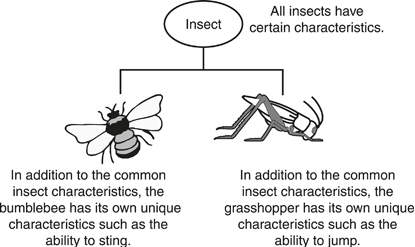
\includegraphics[scale=0.7]{Images/chapter10_section01_inheritInsects.png}
    \end{figure}
\end{frame}

\begin{frame}{Inheritance}
    When one object is a specialized version of another object, there is an ``is a'' relationship between them.
    \begin{itemize}
        \item A \violet{poodle} is a \red{dog}.
        \item a \violet{car} is a \red{vehicle}.
        \item A \violet{flower} is a \red{plant}.
        \item A \violet{rectangle} is a \red{shape}.
    \end{itemize}
    Inheritance involves a \red{superclass} (general class) and a \violet{subclass} (specialized class).
\end{frame}

\begin{frame}[fragile]{Inheritance}
    \begin{lstlisting}[basicstyle=\ttfamily\footnotesize]
public class GradedActivity {
    private double score;
    public void setScore(double s) {
        score = s;
        }
    public double getScore() {
        return score;
        }
    public char getGrade() {
        char letterGrade = 'F';
        if (score >= 90)
            letterGrade = 'A';
        else if (score >= 80)
            letterGrade = 'B';
        else if (score >= 70)
            letterGrade = 'C';
        else if (score >= 60)
            letterGrade = 'D';
        return letterGrade;
        }
    }
    \end{lstlisting}
\end{frame}

\begin{frame}[fragile]{Inheritance}
    Now we can consider different activities that can be graded: quizzes, midterm exams, final exams, lab reports, essays, and so on.
\end{frame}

\begin{frame}[fragile]{Inheritance}
\begin{lstlisting}[basicstyle=\ttfamily\footnotesize]
class FinalExam extends GradedActivity {
	private int numQuestions;
	private int numMissed;
	private double pointsEach;
	public FinalExam(int numQuestions, int numMissed) {
		double numericScore;
		this.numQuestions = numQuestions;
		this.numMissed = numMissed;
		this.pointsEach = 100.0 / numQuestions;
		numericScore = 100.0 - (numMissed * this.pointsEach);
		setScore(numericScore); // pay attention to this line.
		}
	public double getPointsEach() {
		return this.pointsEach;
		}
	public double getNumMissed() {
		return this.numMissed;
		}
	}
\end{lstlisting}
\end{frame}

\begin{frame}[fragile]{Inheritance}
    \begin{lstlisting}
public static void main(String[] args) {
FinalExam exam = new FinalExam(10, 2);
    System.out.println(
        "Each question counts " 
        + exam.getPointsEach()
        + " points.\nThe exam score is "
        + exam.getScore()
        + "\nThe exam grade is "
        + exam.getGrade());
    }
    \end{lstlisting}    
\end{frame}

\begin{frame}{Inheritance}
    \noindent 
    \begin{figure}[H]
    \centering
    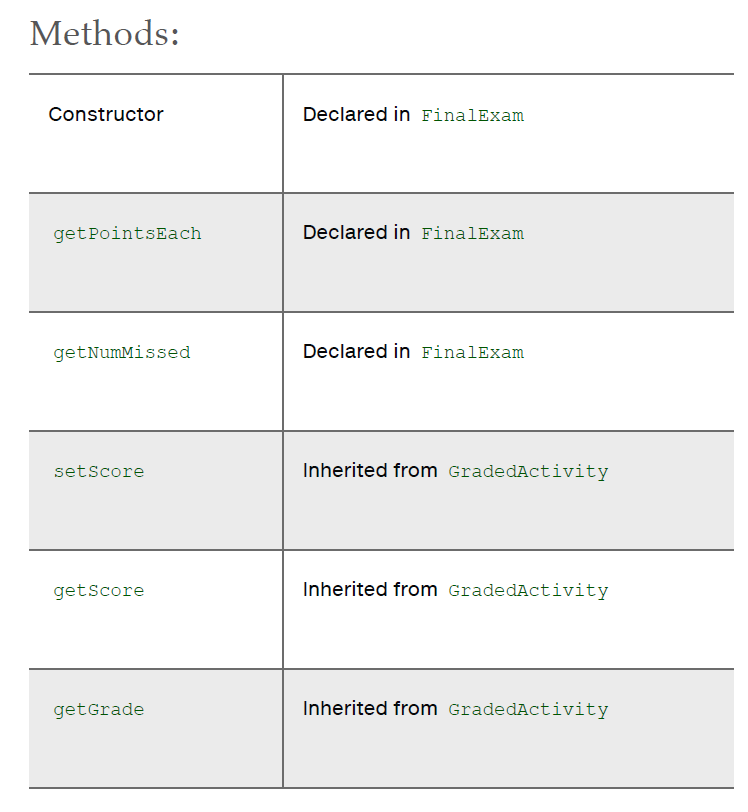
\includegraphics[scale=0.4]{Images/chapter10_section01_listedFcns.png}
    \end{figure}
\end{frame}

\begin{frame}{The Superclass's Constructor}
    In an inheritance relationship, the superclass constructor always executes before the subclass constructor. \\ \vspace{1em}
    The \texttt{GradedActivity} class has only one constructor, which is the default constructor that Java automatically generated for it. \\ \vspace{1em} 
    When a \texttt{FinalExam} object is created, the \texttt{GradedActivity} class’s default constructor is executed just before the FinalExam constructor is executed.
\end{frame}

\begin{frame}[fragile]{The Superclass's Constructor}
    \begin{lstlisting}
public class ConstructorDemo {
    public static void main(String[] args) {
        SubClass obj = new SubClass();
        }
    }
class SuperClass {
    public SuperClass() {
        System.out.println("Superclass constructor.");
        }
    }
class SubClass extends SuperClass {
    public SubClass() {
        System.out.println("Subclass constructor.");
        }
    }
    \end{lstlisting}    
\end{frame}

\subsection{Calling the Superclass Constructor}
\begin{frame}{Calling the Superclass Constructor}
    The \texttt{super} key word refers to an object’s superclass. \\ \vspace{1em}
    You can use the super key word to call a superclass constructor. \\ \vspace{1em}
\end{frame}

\begin{frame}[fragile]{Calling the Superclass Constructor}
\begin{lstlisting}[basicstyle=\ttfamily\footnotesize]
public class SuperDemo {
    public static void main(String[] args) {
        SubClass02 obj = new SubClass02();
        }
    }
class SuperClass02 {
	public SuperClass02() {
		System.out.println("Superclass no-arg constructor.");
		}
	public SuperClass02(int arg) {
		System.out.println(arg + " was passed to the constructor.");
		}
	}
class SubClass02 extends SuperClass02 {
	public SubClass02() {
		super(10); // note use of super.
		System.out.println("Subclass constructor.");
		}
	}
\end{lstlisting}    
\end{frame}

\subsection{Overriding Superclass Methods}
\begin{frame}{Overriding Superclass Methods}
    A subclass may have a method with the same signature as a superclass method. \\ \vspace{1em}
    In such a case, the subclass method overrides the superclass method. \\ \vspace{1em}
    Consider the previous example for \texttt{GradedActivity}, what if we wanted to curve the grades?
\end{frame}

\begin{frame}{Overriding Superclass Methods}
    \noindent 
    \begin{figure}[H]
    \centering
    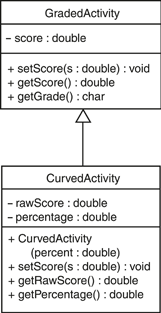
\includegraphics[scale=0.9]{Images/chapter10_section03_curvedActivity.png}
    \end{figure}
\end{frame}

\begin{frame}[fragile]{Overriding Superclass Methods}
\begin{lstlisting}[basicstyle=\ttfamily\footnotesize]
class CurvedActivity extends GradedActivity {
    double rawScore;
    double percentage;
    public CurvedActivity(double percentage) {
        this.percentage = percentage;
        this.rawScore = 0.0;
        }
    @Override
    public void setScore(double score) {
        this.rawScore = score;
        super.setScore(this.rawScore * this.percentage);
        }
    public double getRawScore() {
        return this.rawScore;
        }
    public double getPercentage() {
        return this.percentage;
        }
    }
\end{lstlisting}
\end{frame}

\begin{frame}{Overloading versus Overriding}
    There is a distinction between overloading and overriding.
    \begin{itemize}
        \item Overloading \\
        When a method has the same name as one or more methods but a different parameter list
        \item Overriding \\ 
        When a subclass replaces a method defined in its superclass
    \end{itemize}
\end{frame}

\begin{frame}[fragile]{Preventing a Method from Being Overriden}
    When a method is declared with the \texttt{final} modifier, it cannot be overriden in a subclass.
    \begin{lstlisting}
public final void message()
    \end{lstlisting}
    For example, the compiler will generate an error if a subclass attempts to override the \texttt{message} method.
\end{frame}

\section{Protected Members and Chains of Inheritance}
\subsection{Protected Members}
\begin{frame}{Protected Members}
    So far we have covered two access specifications within a class: \texttt{private} and \texttt{public}. \\ \vspace{1em}
    There exists a third specification: \texttt{protected} with the following properties
    \begin{itemize}
        \item members may be accessed by methods of the same class or a subclass
        \item members may be accessed by methods in any class defined in the same package
        \item overall, the access is a middle ground between \texttt{private} and \texttt{public}.
    \end{itemize}
\end{frame}

\begin{frame}[fragile]{Protected Members}
    \begin{lstlisting}[basicstyle=\ttfamily\footnotesize]
public class ProtectedDemo {
    public static void main(String[] args) {
        GenericClass obj = new GenericClass();
        System.out.println(obj.num);
        obj.printNum();
        }
    }
class GenericClass {
    protected int num = 2023;
    protected void printNum() {
        System.out.println(num);
        }
    }
    \end{lstlisting}
\end{frame}

\begin{frame}[fragile]{Package Access}
    A class member is given package access by default if no access specifier is provided.
    \begin{lstlisting}
public class Circle {
    double radius;
    int centerX, centerY;
    }
    \end{lstlisting}
Note: If a subclass is in a different package, members with package access cannot be accessed.
\end{frame}

\subsection{Chains of Inheritance}
\begin{frame}{Chains of Inheritance}
    It is possible to establish a chain of inheritance.
    \noindent 
    \begin{figure}[H]
    \centering
    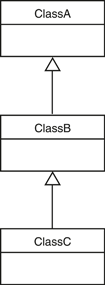
\includegraphics[scale=0.7]{Images/chapter10_section05_chainInheritance.png}
    \end{figure}
\end{frame}

\begin{frame}{Chains of Inheritance}
    Here is a more concrete example.
    \noindent 
    \begin{figure}[H]
    \centering
    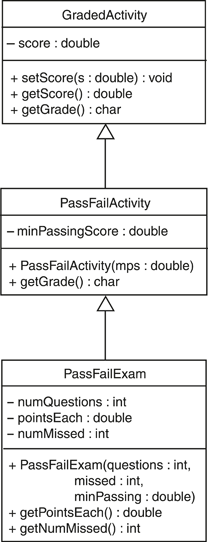
\includegraphics[scale=0.5]{Images/chapter10_section05_chainInheritanceConcrete.png}
    \end{figure}
\end{frame}

\begin{frame}[fragile]{Chains of Inheritance}
    \begin{lstlisting}[basicstyle=\ttfamily\footnotesize]
class GradedActivity {
    private double score;
    public void setScore(double score) {
        this.score = score;
        }
    public double getScore() {
        return this.score;
        }
    public char getGrade() {
        char letterGrade = 'F';
        if (this.score >= 90)
            letterGrade = 'A';
        else if (this.score >= 80)
            letterGrade = 'B';
        else if (this.score >= 70)
            letterGrade = 'C';
        else if (this.score >= 60)
            letterGrade = 'D';
    	return letterGrade;
    	}
    }
    \end{lstlisting}
\end{frame}

\begin{frame}[fragile]{Chains of Inheritance}
    \begin{lstlisting}[basicstyle=\ttfamily\footnotesize]
class PassFailActivity extends GradedActivity {
    private double minPassingScore;
    public PassFailActivity(double minPassingScore) {
        this.minPassingScore = minPassingScore;
        }
    @Override
    public char getGrade() {
        char letterGrade;
        letterGrade = 'F';
        if (super.getScore() >= this.minPassingScore) {
            letterGrade = 'P';
            }
        return letterGrade;
        }
    }
    \end{lstlisting}
\end{frame}

\begin{frame}[fragile]{Chains of Inheritance}
    \begin{lstlisting}[basicstyle=\ttfamily\footnotesize]
class PassFailExam extends PassFailActivity {
    private double pointsEach;
    private int numMissed;
    public PassFailExam(int numQuestions, int numMissed, double minPassing) {
        super(minPassing);
        double numericScore;
        this.numMissed = numMissed;
        pointsEach = 100.0 / numQuestions;
        numericScore = 100.0 - (numMissed * pointsEach);
        setScore(numericScore);
        }
    public double getPointsEach() {
        return this.pointsEach;
        }
    public int getNumMissed() {
        return this.numMissed;
        }
    }
    \end{lstlisting}
\end{frame}

\begin{frame}[fragile]{Chains of Inheritance}
    \begin{lstlisting}[basicstyle=\ttfamily\footnotesize]
class ChainInheritanceDemo {
    public static void main(String[] args) {
        int questions = 100;
        int missed = 25;
        double minPassing = 60;
        PassFailExam exam = new PassFailExam(questions, missed, minPassing);
        System.out.println(
            "Each questions counts " + exam.getPointsEach()
            + " points."
            );
        System.out.println("The exam score is " + exam.getScore());
        System.out.println("The exam grade is " + exam.getGrade());
        }
    }
    \end{lstlisting}
\end{frame}

\section{\texttt{Object} Class and Polymorphism}
\subsection{The \texttt{Object} Class}
\begin{frame}[fragile]{The \texttt{Object} Class}
    The Java API has a class named \texttt{Object}, which all other classes directly or indirectly inherit from. \\ \vspace{1em}
    The class \texttt{Object} is part of the \texttt{java.lang} package. \\ \vspace{1em}
    When a class does not use the \texttt{extends} key word to inherit from another class, Java automatically extends it from the \texttt{Object} class.
    \begin{lstlisting}
public class MyClass {}
// is equivalent to
public class MyClass Extends Object {}
    \end{lstlisting}
\end{frame}

\begin{frame}{The \texttt{Object} Class}
    Since every class extends the \texttt{Object} class, every class inherits the \texttt{Object} class's members. \\ \vspace{1em}

    Two of the most useful are the \texttt{toString} and \texttt{equals} method. \\ \vspace{1em} 

    In the \texttt{Object} class, the \texttt{toString} method returns a reference to a \texttt{String} containing the object's class name, followed by the @ sign, followed by the object's hash code (hexadecimal number). \\ \vspace{1em}

    The \texttt{equals} method accepts a referece to an object as its argument. It returns \texttt{true} if the argument references the calling object.
\end{frame}

\begin{frame}[fragile]{The \texttt{Object} Class}
    \begin{lstlisting}[basicstyle=\ttfamily\footnotesize]
public class ObjectMethods {
    public static void main(String[] args) {
        GenericClass obj = new GenericClass();
        GenericClass obj1 = new GenericClass();
        System.out.println(obj);
        System.out.println(obj1);
        System.out.println(obj.equals(obj1));
        }
    }
class GenericClass {
    int num = 1;
    void getNum() {
        System.out.println(this.num);
        }
    }
    \end{lstlisting}
\end{frame}

\subsection{Polymorphism}
\begin{frame}[fragile]{Polymorphism}
    A superclass reference variable can reference objects of a subclass. \\ \vspace{1em}
    So far we have defined reference variables in the following manner
    \begin{lstlisting}
GradedActivity exam = new GradedActivity();
    \end{lstlisting}
    Previously, we have defined two subclasses of \texttt{GradedActivty}: \texttt{PassFailActivity} and \texttt{PassFailExam}. \\ \vspace{1em}
    This allows us to write the following
    \begin{lstlisting}
GradedActivity exam1 = new FinalExam(50, 7);
GradedActivity exam2 = new PassFailActivity(70);
GradedActivity exam3 = new PassFailExam(100, 10, 70);
    \end{lstlisting}
\end{frame}

\begin{frame}[fragile]{Polymorphism}
    The term \textit{polymorphism} means the ability to take many forms. \\ \vspace{1em}
    In Java, a reference variable is polymorphic because it can reference objets of types different from its own, as long as those tpyes are subclasses of its type. \\ \vspace{1em}
    Note there are some limitations:
    \begin{lstlisting}
GradedActivity exam = new PassFailExam(100, 10, 70);
System.out.println(exam.getScore());        // Works.
System.out.println(exam.getGrade());        // Works.
System.out.println(exam.getPointsEach());   // ERROR
    \end{lstlisting}
\end{frame}

\begin{frame}[fragile]{Polymorphism and Dynamic Binding}
    Consider the following:
    \begin{itemize}
        \item a superclass variable references a subclass object
        \item the subclass has overriden a method in the superclass
        \item the superclass reference variable makes a call to the overriden method
        \item which method is called?
    \end{itemize}
    \begin{lstlisting}
GradedActivity exam = new PassFailActivity(60);
exam.setScore(70);
System.out.println(exam.getGrade()); // example of dynamic binding
    \end{lstlisting}
\end{frame}

\begin{frame}{Polymorphism and Dynamic Binding}
    The process of matching a method call with the correct method definition is known as binding. \\ \vspace{1em} 
    Java performs dynamic binding when a variable contains a polymorphic reference. \\ \vspace{1em} 
    The JVM determines at runtime which method to call, \red{depending on the type of object that the variable references}.
\end{frame}

\begin{frame}[fragile]{Polymorphism and Dynamic Binding}
    You can also use parameters to accept arguments to methods polymorphically:
    \begin{lstlisting}
public static void displayGrades(GradedActivity actObj) {
    System.out.println("Score " + actObj.getScore()
        + " , grade " + actObj.getGrade()
        );
    }
    \end{lstlisting}
    Which allows for
    \begin{lstlisting}
GradedActivity exam1 = new FinalExam(50, 7);
GradedActivity exam2 = new PassFailACtivity(70);
GradedActivity exam3 = new PassFailExam(100, 10, 70);
displayGrades(exam1);
displayGrades(exam2);
displayGrades(exam3);
    \end{lstlisting}
\end{frame}

\begin{frame}[fragile]{Polymorphism and Dynamic Binding}
    The \texttt{Is-a} relationship does not work in reverse. \\ \vspace{1em}
    For example: all seniors are students but not all students are seniors. \\ \vspace{1em}
    In Java, you want to avoid writing:
    \begin{lstlisting}
GradedActivity activity = new GradedActivity();
Final exam = activity; // ERROR
    \end{lstlisting}
\end{frame}

\begin{frame}[fragile]{The \texttt{instanceof} Operator}
    There is an operator in Java named \texttt{instanceof} to determine whether an object is an instance of a particular class.
    \begin{lstlisting}
GradedActivity activity = new GradedActivity();
FinalExam exam = new FinalExam(20, 2);
boolean x, y;
x = activity instanceof GradedActivity; // true
y = exam instanceof GradedActivity;     // true
    \end{lstlisting}
\end{frame}

\section{Abstract Classes, Abstract Methods and Interfaces}
\subsection{Abstract Classes and Methods}
\begin{frame}[fragile]{Abstract Classes and Abstract Methods}
    An abstract class is not instantiated, but other classes extend it. \\ \vspace{1em}
    An abstract method has only a header and no body. \\ \vspace{1em}
    \begin{lstlisting}
public abstract void setValue(int value);
    \end{lstlisting}
    When an abstract method appears in a class, the method must be overriden in a subclass otherwise an error will result.
\end{frame}

\begin{frame}{Abstract Classes and Abstract Methods}
    When a class contains an abstract method, you cannot create an instance of the class. \\ \vspace{1em}

    An abstract class represents the generic or abstract form of all the classes that inherit from it. \\ \vspace{1em}

    A class becomes abstract when you place the \texttt{abstract} key word in the class definition
\end{frame}

\begin{frame}[fragile]{Abstract Classes and Abstract Methods}
    \begin{lstlisting}[basicstyle=\ttfamily\footnotesize]
abstract class Student {
    private String name, idNumber;
    private int yearAdmitted;
    public Student(String name, String idNumber, int yearAdmitted) {
        this.name = name;
        this.idNumber = idNumber;
        this.yearAdmitted = yearAdmitted;
        }
    public String toString() {
        String str;
        str = "Name: " + this.name
            + "\nID Number: " + this.idNumber
            + "\nYear Admitted: " + yearAdmitted;
        return str;
        }
    public abstract int getRemainingHours();
    }
    \end{lstlisting}    
\end{frame}

\begin{frame}{Abstract Classes and Abstract Methods}
    See lecture video for demo on extending the abstract Student class.
\end{frame}

\begin{frame}{Abstract Classes and Abstract Methods}
    In summary,
    \begin{itemize}
        \item Abstract methods and abstract classes are defined with the \texttt{abstract} key word.
        \item Abstract methods have no body, and their header must end with a semicolon.
        \item An abstract method must be overriden in a subclass.
        \item When a class contains an abstract method, it cannot be instantiated. It must serve as a superclass.
        \item An abstract class cannot be instantiated. It must serve as a superclass.
    \end{itemize}
\end{frame}

\subsection{Interfaces}
\begin{frame}[fragile]{Interfaces}
    An interface specifies behavior for a class. \\ \vspace{1em}
    In its simplest form, an interface is like a class that contains only abstract methods. \\ \vspace{1em}
    An interface cannot be instantiated, it is \textit{implemented} by other classes. \\ \vspace{1em}
    When a class implements an interface, the class must override the methods that are specified by the interface.
    \begin{lstlisting}
public interface Displayable {
    void display();
    // more method headers
    // all methods are implicitly public
    }
    \end{lstlisting}
\end{frame}

\begin{frame}[fragile]{Interfaces}
    \begin{lstlisting}
public class Person implements Displayable {
    private String name;
    public Person(String name) {
        this.name = name;
        }
    public void display() {
        System.out.println("My name is " + name);
        }
    }
    \end{lstlisting}
\end{frame}

\begin{frame}[fragile]{Interfaces}
    When a class implements an interface, it is agreeing to provide all of the methods that are specific by the interface.
    \begin{lstlisting}
interface Relatable {
    boolean equals(GradedActivity g);
    boolean isGreater(GradedActivity g);
    boolean isLess(GradedActivity g);
    }
    \end{lstlisting}
\end{frame}

\begin{frame}[fragile]{Interfaces}
    \begin{lstlisting}[basicstyle=\ttfamily\footnotesize]
class ChainInheritanceDemo {
    public static void main(String[] args) {
        FinalExam3 exam1 = new FinalExam3(100, 20);
        FinalExam3 exam2 = new FinalExam3(100, 30);
        System.out.println("Exam 1: " + exam1.getScore());
        System.out.println("Exam 2: " + exam2.getScore());
        if (exam1.equals(exam2)) {
            System.out.println("The exam scores are equal.");
            }
        if (exam1.isGreater(exam2)) {
            System.out.println("The Exam 1 score is the highest.");
            }
        if (exam1.isLess(exam2)) {
            System.out.println("The Exam 1 score is the lowest.");
            }
        }
    }
    \end{lstlisting}
\end{frame}

\begin{frame}[fragile]{Interfaces}
    An interface can contain field declarations, but all fields in an interface are treated as \texttt{final} and \texttt{static}.
    \begin{lstlisting}
public interface Doable {
    int FIELD1 = 1;
    int FIELD2 = 2;
    // some method headers go here
    }
    \end{lstlisting}
    In this interface, \texttt{FIELD1} and \texttt{FIELD2} are \texttt{final static int} variables. Any class that implements this interface has access to these variables.
\end{frame}

\begin{frame}[fragile]{Interfaces}
    A Java class can extend only one superclass but implement multiple interfaces. \\ \vspace{1em}
    When a class implements multiple interfaces, it must provide the methods specified by all of them.
    \begin{lstlisting}[basicstyle=\ttfamily\footnotesize]
public class MyClass implements Interface1, Interface2, Interface3
    \end{lstlisting}
\end{frame}

\end{document}